
%\section{USER STUDY}
%There are two studies.
%The purpose of the study is to determine users� ability to provide 2D input using FingerPad. 


%Two usage conditioned were included: seated and walking.
%Our goal was to understand how precise the participants can perform cursor control on the move.


\subsection{USER STUDY: SEATED VS. WALKING}
The purpose of the study is to determine users� ability to provide precise cursor control through the pinched fingertips. We performed the task under two conditions: seated and walking conditions. 
%The seated condition allows us to see how well participants used our techniques after training. 
The walking condition allows us to see the level of influence when using FingerPad technique on the move with glass displays.
%The walking condition reveals the level of influence from walking waving.
%A questionnaire followed the study.

%native user ability in cursor control because the button-press minimizes  the errors from commitment methods. 
\subsection{Task}
Participants moved the cursor over the target and committed using a remote clicker in the non-dominant hand. 
The target changed color when the cursor entered the target square. 
Upon successful selection, the target disappeared and next target showed up.
We measured task time and error rate for target sizes of 11mm, 5.5mm, 2.8mm, 1.4mm and 0.6mm by side. The 0.6mm case is included to test the user limitation.

\begin{figure}
\begin{center}
  \begin{tabular}{@{\hspace{0.1cm}}c}
		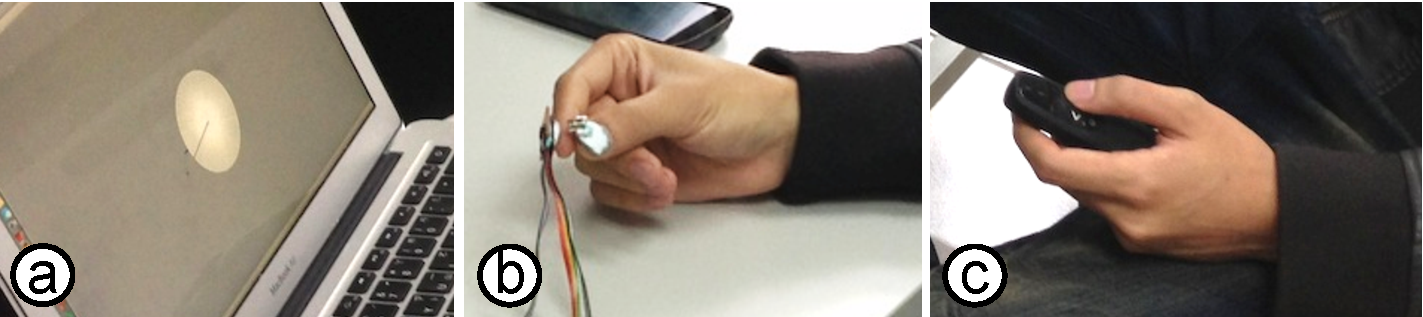
\includegraphics[width=1\linewidth]{seated2}\\
   \end{tabular}
\caption{The setup of our user study. (a) The screen, (b) the FingerPad device, and (c) the clicker in the non-dominant hand.}
\label{fig:seated}
\end{center}
\end{figure}

\subsection{Conditions}
In the \emph{seated condition}, participants sat on the chair in front of the table where the screen was positioned toward the user. They were instructed to adjust the chair height such that they could rest their dominant hands on the table for support (Figure \ref{fig:seated}a). In order to make sure they could see the smallest 0.6mm target clearly, the screen was repositioned to about 30 cm to the participants' eyes.

In the \emph{walking condition}, they performed the tasks on the treadmill. The screen was placed on top of the treadmill control platform, as shown in Figure \ref{fig:walking}.
We set the speed to 3.5 km per hour, with a range of 0.5km according to the participants.

%\subsection{USER STUDY 1: PRECISION TASK}
%The purpose of the study is to determine users� ability to provide precise cursor control using the pinched fingertips. We performed the precision task with two commitment methods: single-handed flick and bimanual button-press. 
%The single-handed condition allows us to see how well participants used our techniques after training. The bimanual condition reveals native user ability in cursor control because the button-press minimizes  the errors from commitment methods. A questionnaire followed the study.

%Participants were instructed to perform target acquisition tasks. 
%The study were tested under two commitment methods: single-handed flick and bimanual click. 

%\subsection{Task}
%Participants were asked to perform precision tasks. 
%Participants moved the cursor over the target and committed using single-handed flick or bimanual button press, depending on interface condition. 
%The target changed color when the cursor entered the target square. %When satisfied with their selection, participants committed by flicking the thumb up in the single-handed condition (Figure) or by pressing the button in their non-dominant hand in the bimanual condition (Figure).
%Upon successful selection, the target disappeared and next target showed up.
%We measured task time and error rate for target sizes of 11mm, 5.5mm, 2.8mm, 1.4mm and 0.6mm by side. 

\begin{figure}
\begin{center}
  \begin{tabular}{@{\hspace{0.1cm}}c}
		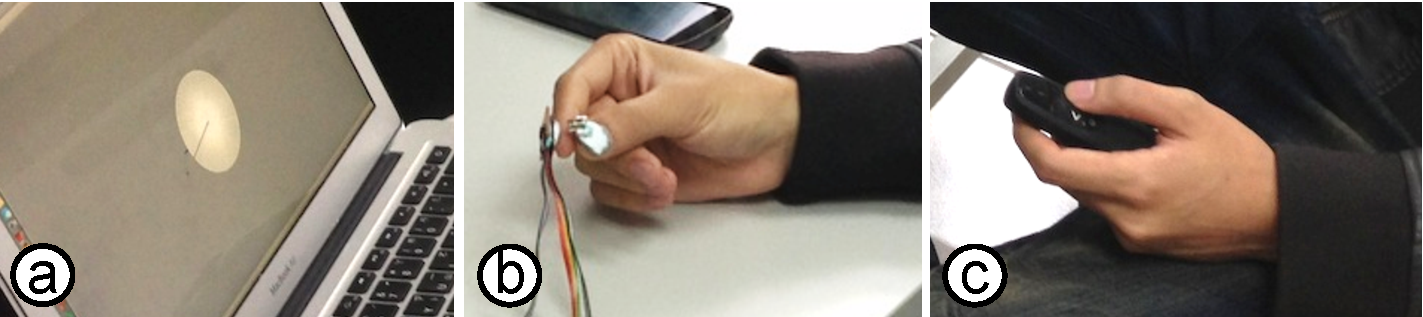
\includegraphics[width=1\linewidth]{seated2}\\
   \end{tabular}
\caption{The setup of our user study. (a) The screen, (b) the FingerPad device, and (c) the clicker in the non-dominant hand.}
\label{fig:seated}
\end{center}
\end{figure}

\subsection{Conditions}
In the \emph{single-handed condition}, participants committed a selection by flicking the thumb up. 
This is similar to take-off selection. As described in PROTOTYPE, we set the canceling window to 120ms.  Participants were trained to become familiar with the flicking-up gesture, making sure they adapted well to the optimal flicking speed in the training phase. They have to perform less than three errors in consecutive 12 tasks, including all target sizes. 

In the \emph{bimanual condition}, participants committed by pressing a wireless clicker in the non-dominant hand.
We include the bimanual condition, in order to remove errors introduced by flicking detection. 
This condition allows us to see the upper bound of user performance in cursor control.

%Because the speed of the gesture performed affected resulting committed cursor position.
%At the moment the flicking-up selection detected, we remove the last 100ms cursor movement. 


%If participants were not able to  perform flicking gesture well, they were instructed to move apart the pinched fingertips as fast as possible.

\subsection{Interface  and apparatus}
Participants worn the sensor part of the finger pad device on the index fingernail, and the magnet part on the thumbnails. Because the nail sizes and the way participants move their thumbs on the index finger pads are bio-mechanically different, we helped participants put on the device, and adjusted the magnet such that the magnet orientation was parallel to the normal of the sensor gird when tapping the thumb in the center of the index finger pad.
In addition, we used a larger magnet (4mm disk * 8mm height), the stronger magnetic field improves cursoring stabilization and makes sure participants with thicker fingertips work well too.




\subsection{Experimental design}
%The experiment was a 5x2 within-subjects factorial design, with five button size conditions ( 11mm, 5.5mm, 2.8mm, 1.2mm, 0.6mm), and two commitment conditions (single-handed flick and bimanual click).
The experiment was within-subjects. The study design was 2 x 5 x 12 (Commit method x Target Size x Target Position) with 3 repetitions for each cell. 
Target sizes were 11mm, 5.5mm, 2.8mm, 1.4mm and 0.6mm by side; target positions were the 12 centroids of a regular 4 x 3 grid. 
For each trial, we recorded task completion time and error. Commit method was counterbalanced. Target sizes and positions were randomized. %Participants received up-front training.

\subsection{Participants}
15 volunteers, (8 female) between the ages of 22 and 40 were recruited from the university. Each was gifted a pack of chocolate for their time. All participants were using touch-input smart phones. All were right-handed.

\subsection{Results and discussion}
show result and discuss here.

\subsection{USER STUDY 2: WALKING}
In study 2, we tested this ability under walking condition, with the bimanual button-press as the only commitment method. Interface, apparatus and task design were same as Study 1, except that we only tested bimanual button-press. The study design was 5 x 12 (Target Size x Target Position) with 3 repetitions for each cell. 

\subsection{Apparatus}
Participants were instructed to perform precision tasks on the treadmill. The treadmill was set to normal walking speed (5.0 km/hour). The screen was positioned on the treadmill such that the participants can see it clearly when walking on the  treadmill platform.

\subsection{Participants}
15 volunteers, (8 female) between the ages of 22 and 40 were recruited. Each was gifted a pack of chocolate for their time. All were right-handed.

\begin{figure}
\begin{center}
  \begin{tabular}{@{\hspace{0.1cm}}c}
		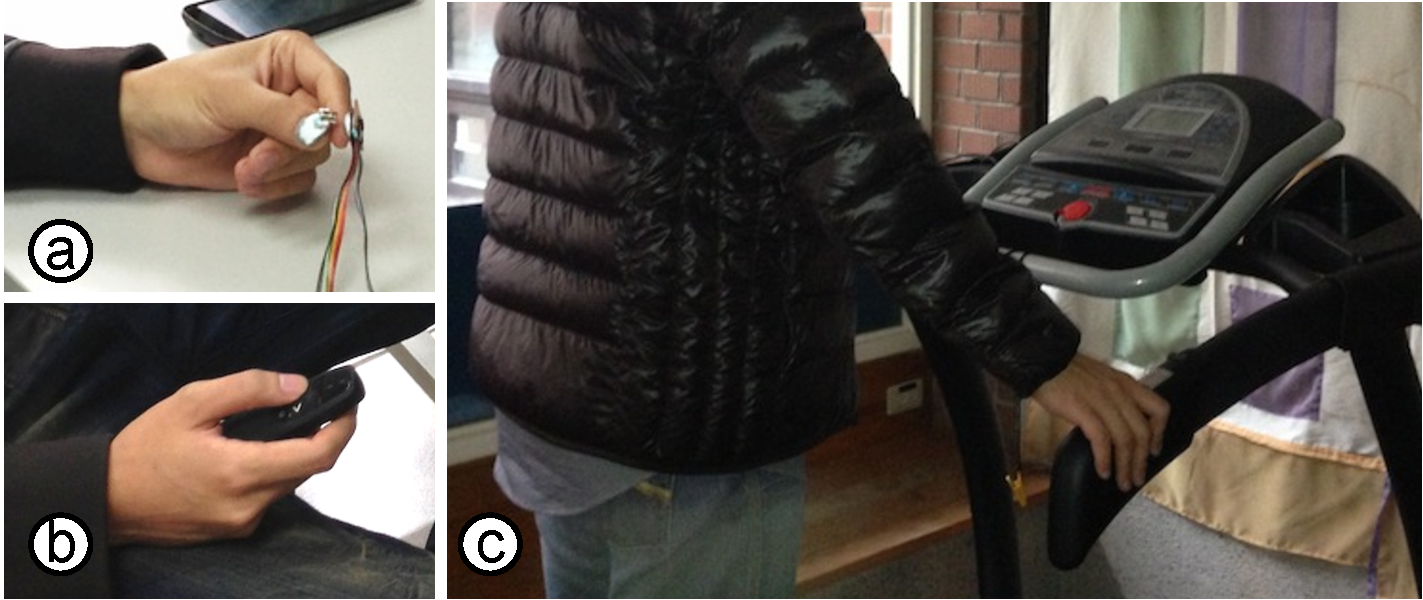
\includegraphics[width=1\linewidth]{walking}\\
   \end{tabular}
\caption{Walking study.}
\label{fig:walking}
\end{center}
\end{figure}

\subsection{Results and discussion}
result shows here.


\subsubsection{Commitment method}

\begin{figure}
\begin{center}
  \begin{tabular}{@{\hspace{0.1cm}}c}
		\includegraphics[width=1\linewidth]{clickMethods}\\
   \end{tabular}
\caption{Other commitment methods described by the participants. (a) press (e.g., button), (b) move the middle finger, (c) tap the thumb pad with middle finger, and (d) move the wrist. The white regions highlight the moving part of the gestures performed.}
\label{fig:clickMethods}
\end{center}
\end{figure}



%\section{STUDY 1: INDEXPAD and THUMBPAD}
%The goal of the study is to understand the roles of index finger and thumb in FingerPad. 
%What are suitable applications participants could think of?
%Identified some many different potentials of IndexPad and ThumbPad, so that we could only focus on one particular model, the IndexPad.
%The result pushes us toward deep investigation into IndexPad.
%The study of ThumbPad is, therefore, not in the scope of this paper.


%\subsection{Explorative Study}


